\section{Введение}

Одна из основных задач, стоящих перед разработчиками и исследователями в области анимации, -- это воспроизведение разнообразия движений человека, с целью  создания персонажей, способных реалистично взаимодействовать с игровым миром. Несмотря на сложности, связанные с недостаточным пониманием всех тонкостей движения человека, множество подходов к решению этой задачи было предложено за последние десятилетия. Существующие подходы можно разделить на две группы: основанные на данных и основанные на физическом моделировании. Первая группа использует большое количество предварительно записанных движений человека, для создания необходимых анимаций персонажа. Такие подходы демонстрируют хорошие результаты, поскольку полагаются на данные собранные в реальном мире, однако плохо применимы в случае когда требуемое движение не стандартно и не похоже на имеющиеся. Вторая группа управляет динамикой физической модели персонажа. В таком случае обеспечивается физическая корректность и появляется возможность взаимодействия с виртуальной средой.

Широко распространенная проблема управления -- это поддержание баланса при движении, то есть предотвращение падения персонажа. Особенно ярко проблема проявляется, когда персонаж находится в присутствии внешних возмущений или на неровной поверхности. В данной работе описывается способ поддержания баланса персонажа следующего опорной анимации на основе локальной оптимизации и маркеров сбалансированности, предложенных в \cite{MacchiettoZS}. В каждый момент времени решается задача квадратичного программирования, которая оптимизирует значения целевых функций, отвечающих за баланс и следование за анимацией. После персонаж приводится в движение в соответствии с результатами оптимизации. Более того, при изменение целевых функций описываемый способ может быть адаптирован для других проблем управления.

\subsection{Модель персонажа}

Перед тем как перейти к описанию разработанной системы, построим физическую модель персонажа и сформулируем уравнения, описывающие ее.

\subsubsection{Кинематическое дерево}

\begin{figure}
  \begin{minipage}[t]{0.475\textwidth}
    \centering
    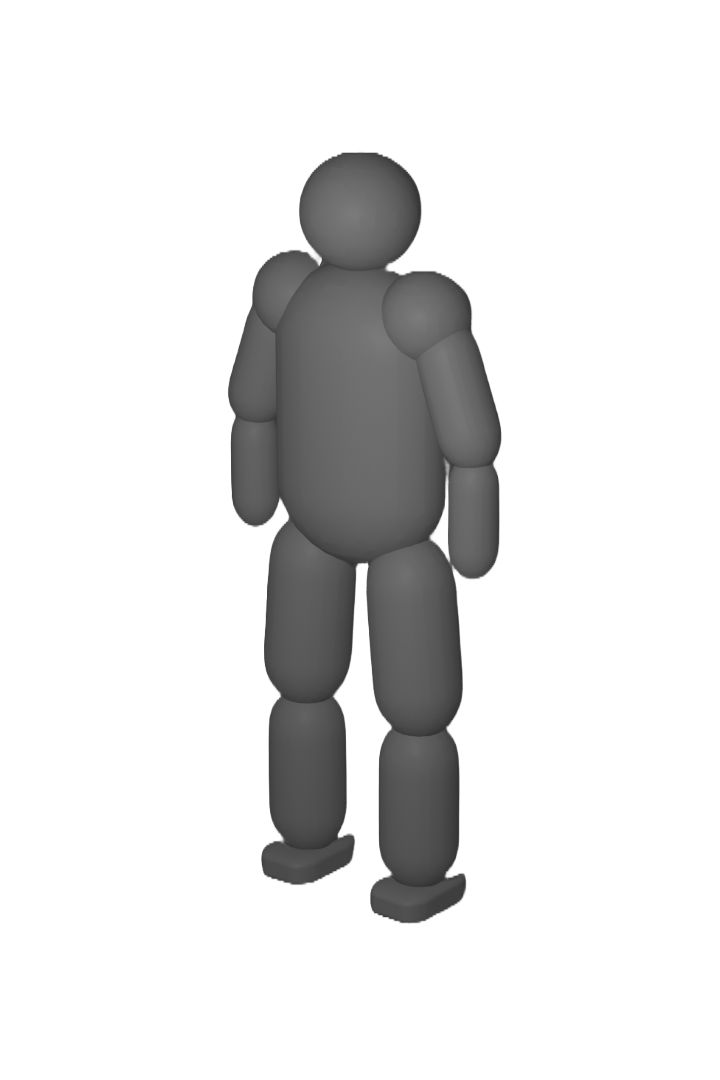
\includegraphics[scale=0.25]{visual_model.png}
    \caption{Трехмерная модель}
    \label{image:visual_model}
  \end{minipage}
\hfill
  \begin{minipage}[t]{0.475\textwidth}
    \centering
    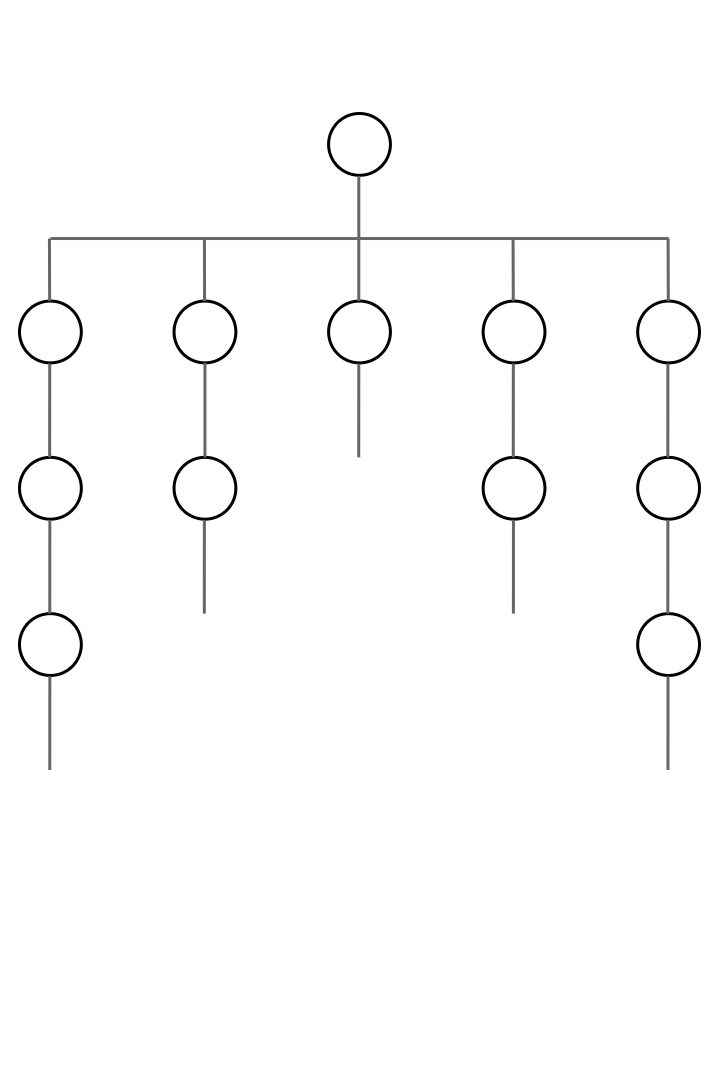
\includegraphics[scale=0.25]{kinematic_tree.png}
    \caption{Кинематическое дерево. Круги обозначают шарниры, а соединения между кругами -- твердые тела}
    \label{image:kinematic_tree}
  \end{minipage}
\end{figure}

Кинематическое дерево -- это система из $n$ твердых тел, соединенных между собой $m$ шарнирами. Каждый из шарниров, кроме корневого, ограничивает относительное движение тел, которые он соединяет. Например, призматический шарнир оставляет только поступательное движение вдоль выбранной оси. Корневой шарнир, в свою очередь, определяет возможность системы перемещаться в пространстве и бывает двух видов: плавающий, то есть не накладывающий ограничений, и фиксирующий.

Для того чтобы приводить в движение отдельные тела, некоторые шарниры могут быть снабжены приводами, которые генерируют необходимые силы и моменты сил. В таком случае шарнир называется активным, иначе, соответственно, неактивным. Отметим, что корневой шарнир обычно остается без привода. Таким образом за движение системы как целого отвечает сила трения, что сохраняет физическую корректность, но сильно усложняет управление кинематическим деревом.

В данной работе персонаж моделируется как кинематическое дерево, все шарниры которого имеют привод, причем силы и моменты сил, генерируемые в корневом шарнире, минимизируются в оптимизаторе. Такая модель в большинстве ситуаций эквивалентна кинематическому дереву с неактивным корневым шарниром, однако оставляет возможность нарушить физическую корректность при необходимости. На рисунках \ref{image:visual_model} и \ref{image:kinematic_tree} изображен пример трехмерной модели персонажа и соответствующего кинематического дерева.

\subsubsection{Обобщенные координаты}

При работе с кинематическим дерево важную роль играет способ, выбранный для описания положения и ориентации тел в пространстве, поскольку он во многом определят простоту, устойчивость и вычислительную сложность моделирования. Основные способы -- это максимальные координаты и обобщенные координаты.

Максимальные координаты описывают тела по отдельности, используя по 6 чисел на каждое, а ограничения, накладываемые шарнирами, учитывают при решении уравнения динамики. Такой способ позволяет использовать существующие системы физического моделирования, но страдает от ошибок работы с вещественными числами, которые приводят к тому, что тела открепляются друг от друга.

Обобщенные координаты, напротив, учитывают связи между телами. Например, для кинематического дерева, состоящего из двух тел, соединенных вращательным шарниром, используется 7 чисел, первые 6 из которых описывают положение и ориентацию одного из тел, а оставшееся -- угол поворота вокруг оси шарнира. Такой способ минимизирует количество используемых чисел и неявно учитывает ограничения.

В данной работе используются обобщенные координаты, скорости и ускорения. Отметим, что обобщенные скорости позволяют выразить скорость любого шарнира. Для этого необходимо умножить их на якобиан шарнира. После чего можно получить скорость любой точки твердого тела, прикрепленного к шарниру, зная ее положение.

\subsubsection{Уравнение динамики}

Уравнение динамики кинематического дерева, может быть выведено из принципа наименьшего действия, и имеет вид
\[
H(q) \ddot{q} + C(q, \dot{q}) + G(q) = u + J(q)^{T} f,
\]
где $q, \dot{q}, \ddot{q}$ -- обобщенные координаты, скорости и ускорения, $H$ -- матрица инерции, $C$ -- центробежная и кориолисова силы, $G$ -- сила тяготения, $u$ -- силы генерируемые приводами, $J$ -- якобиан, и $f$ -- внешние силы.

В качестве неизвестной в этом уравнении может выступать $\ddot{q}$ или $u$. Алгоритмы, который находят $\ddot{q}$, называются алгоритмами прямой динамики. В данной работе используется алгоритм articulated rigid body, описанный в \cite{Featherstone}, который в сравнении с численными методами решения уравнений обладает меньшей вычислительной сложностью.

% NOTE: We can spill more water here. Talk about H and C and G computations.

\subsubsection{Центроидальная матрица}

В разработке систем управления персонажем активно используются такие величины как импульс и момент импульса кинематического дерева. Например, в \cite{MacchiettoZS} показана их тесная связь с маркерами баланса.

В \cite{OrinG} показана связь импульса и момента импульса, выраженных в неподвижной системе отсчета, расположенной в центре масс кинематического дерева, с обобщенными скоростями, имеющая следующий вид
\[
\begin{pmatrix} P\\ L \end{pmatrix} = A(q) \dot{q},
\]
где $P$ -- импульс, $L$ -- момент импульса, а $A$ -- это центроидальная матрица.

Центроидальная матрица, как и матрицей инерции, является фундаментальной характеристикой кинематического дерева, которая зависит только от массы, инерции и значения обобщенных координат твердых тел, составляющих его.
